% !TeX root = ../Bachelorarbeit.tex
\chapter{Einleitung}

\section{Motivation}
Die Motivation für die Erarbeitung der Forschungsfrage ergab sich am 19. Juli 2020, als eine Rundmail des Data Breach Monitoring-Tools von Firefox die Bildschirme erreichte, welches einen neuen Incident bei Wattpad meldete [A16]. Nun stellt sich die berechtigte Frage, inwiefern diese in Relation kleine Webseite verwertbare Daten für einen Angreifer oder ein bösartiges Tool liefern kann. Dazu genügt es sich die Daten genauer anzusehen. Kompromittiert wurden neben den klassichen Daten wie Passwörtern, IP-Adressen, E-Mail-Adressen und Geburtsdaten auch sehr persönliche Informationen wie geografische Standorte, ein Kurzprofil des Nutzers und die Social-Media-Profile der Nutzer [A16]. Entnehmen kann man dies mehreren Artikeln, bei der die Angabe nach der Größe der Datenmengen zwischen 250 und 280 Millionen Einträgen variiert [A17, A18]. Eine genaue Zahl liefert der Artikel der riskbasedsecurity mit 268.830.266 (nach der Entfernung von Duplikaten) kompromittierten E-Mail Addressen, die sich laut des Artikels in einer einzigen Datenbank befanden \cite{A6}. Diese Zahl ist dennoch nur als Richtwert zu verstehen, da das Ausmaß des Datenlecks bei Wattpad nicht in Gänze bekannt ist.

\section{Problemdefinition}
Mit dem Passwort gelangt der Angreifer an die Identität des Nutzers.  Identitätsdiebstahl sei laut BSI ein alltägliches Phänomen, dass jeden Monat eine große Anzahl an digitalen Identitäten von Privatanwendern betrifft [A19]. Es ist allgemein bekannt, dass Daten die im Internet landen kaum oder nur mit erheblichem Mehraufwand aus diesem vollständig entfernbar sind. Die Identität kann nun für missbräuchliche Zwecke entfremdet und missbraucht werden.
\newpage

Auch wenn es bei der Bekanntmachung und Berichterstattung zu solchen Datenlecks manchmal so scheint, ist auch dieses nicht das einzige Beispiel für kompromittierte Unternehmen der letzten Jahre. Angriffsszenarien auf technischer Seite (Code-Injektionen, 0-Day-Exploits, Bruteforce-Angriffe) scheint die informationsaffine Menscheit der Neuzeit gut organisiert zu bekommen, doch dann scheitert es in riesigen Unternehmen oft an der Wahl eines Passwortes einer wichtigen Einzelperson, welches dann in Kettenreaktionen zu solchen Data Breaches führen. Passwörter wichtiger Personen innerhalb eines Unternehmens können nun ohne große Mühen über die Google Suchergebnisse gefunden werden. So liefert die Anfrage 'allintext:password filetype:log after:2019' auf Google alle Logdateien nach 2019, die den Schlüssel ``password'' beeinhalten. Alternativ kann man  über Anfragen folgender Art: 'wattpad data breach download' gezielt nach einem Downloadlink für spezielle Data Breaches suchen. Solche Listen werden häufig in unbekannteren Foren geteilt. Meistens erscheinen Username und Passwort im Format 'Username:Passwort', der erste Doppelpunkt trennt demnach die beiden Zeichenketten. Der Zeilenumbruch trennt die unterschiedlichen Accounts.

Bei Disskusionen im Internet, wird sich häufig aufgrund der selben (wiederholenden) Gründe gegen eine \ac{2fa} und zusätzliche Sicherheiten für die Passwortwahl ausgesprochen. Zum Einen sei ein Verlust des Gerätes, mit dem die Webseite gekoppelt ist, gleichzustzen mit dem Verlust der Identität. Ohne entsprechende Backup-Codes kann womöglich kein Zugang mehr gewährt werden, da das Zurücksetzen des Passwortes meist auch die Authentifizierung durch den zweiten Faktor benötigt. Außerdem spielt die Bequemlichkeit eine große Rolle. Ein User will so schnell wie möglich und ohne Zwischenschritte Zugang zu seinen Diensten erhalten. Ein zweiter Faktor bedeutet das nach Eingabe des Passwortes das Smartphone gesucht, womöglich noch entsperrt, die zugehörige App geöffnet und der Code (PIN, Fingerabdruck, Gesichtsmerkmale) an den Server übertragen und verarbeitet werden muss.

Das Speichern von allen Passwörtern, durch einen Passwort-Manager, an einem gesammelten Ort erscheint dem Durchschnitznutzer als zu riskant. Der Verlust des Masterpasswortes würde den Verlust aller Identitäten des Nutzers bedeuten, sofern er die Daten nicht auswendig kennt oder sich anderweitig notiert hat. Das potenzielle Risiko welches durch verstreute Passwörter im Vergleich zu den Risiken neuerer Verfahren aufkommt, wird häufig ignoriert. Die Frage, die sich stellt ist es, ob man mit einer Kombination aus den vorhandenen vielfältigen Authentifizierungsmöglichkeiten eine bequeeme aber gleichzeitig sichere Authentifizierungsvariante schaffen kann, bei denen es dem Anwender möglich sein soll, sich gegenüber einer Webseite zu authentifizieren.

\section{Stand der Forschung}
\subsection{Bequemlichkeitsproblem}
Bei einem Angriff ist es nicht zwingend notwendig, dass die Authentifizierungsquelle, also jene Quelle bei der die Daten persistiert sind und die die Authentifizierung bei Eingabe durchführt, diese Daten durch fehlerhafte Programmierung herausgibt. Durch sogenannte Metadaten, das sind Informationen und Merkmale zu Daten, ist es Angreifern häufig möglich das Passwort zu erraten bzw. zurückzusetzen. Wenn also der Benutzername lautet 'MichaelJacksonFanForever' ist die Antwort auf die Sicherheitsfrage zum Lieblingskünstler nicht weit entfernt.

Gleichzeitig neigen Menschen aufgrund von Bequemlichkeit zu leicht merkbaren Passwörtern, die sie mehrfach für verschiedene Dienste verwenden. Dies stützt eine kürzlich durchgeführte repräsentative Studie der Bitkom Reserach \cite{A1} im Auftrag des Digitalverbands Bitkom. So nutze etwa jeder dritte Onlinenutzer (36\%) dasselbe Passwort für mehrere Dienste. Auch wenn gleichzeitig 63\% der Befragten angaben, bei der Erstellung von Passwörtern auf ``einen Mix aus Buchstaben, Zahlen und Sonderzeichen'' zu achten, beweist diese Befragung an 1.000 Internetznutzern, dass die Frage nach der Sicherheit von Passwörtern auch im Jahre 2020 immernoch Relevanz hat. Eine ähnliche Studie hat die Bitkom zum Thema 'Nachlässigkeit bei Passwörtern' am 08.11.2016 \cite{A2} gemacht, bei der die prozentuale Verteilung an unsicheren Passwortnutzern die befragt wurden nur einen Prozent höher liegt. Das heißt konkret, dass sich innerhalb von 4 Jahren keine messbare Besserung ergeben hat. Das Bewusstsein über die Internetpräsenz und der Schutz dessen scheinen immernoch keine große Aufmerksamkeit vom modernen Nutzer zu erhalten. Das Problem mit unsicheren Passwörtern ist allerdings so alt wie das Internet.

\subsection{Unsichere Passwörter}
In der fünften Ausgabe der Zeitschrift ``Wirtschaftsinformatik \& Management''  2018 mit dem Titel ``Schwache Passwörter - Nutzer spielen weiterhin Vogel Strauß'' schrieb der Autor Geralt Beuchelt: ``Der Umgang mit Passwörtern ist so ähnlich wie eine Diät: Eigentlich weiß man genau, was richtig ist - Macht aber oft genug das Gegenteil. Und nicht selten ist der Grund Bequemlichkeit. Warum selber kochen, wann nach einem langen Tag eine Pizza lockt? Und warum lange, umständliche Passwörter verwenden, wenn es einfach zu merkende, die man für alle Accounts verwendet, doch auch tun?'' \cite{A3}.
\newpage

Damit greift der Autor sehr zutreffend die Hauptproblematik des Passwortes in der Neuzeit auf. Die symbolische Pizza steht für die Mehrfachverwendung von teils schwachen Passwörtern für alle genutzten Dienste inklusive des 'Verwaltungsdienstes' wie der Mail, welches als meist einziges Identifikationsmerkmal dient, über die weitere Dienste betroffen sein können. Der Begriff des Passwortes stammt aus dem militärischen Bereich des 16. Jahrhunderts, wobei tatsächlich das einzelne Wort adressiert war, welches einem Zutritt zu Gebäuden verschaffte. Damit verwandt ist das Kennwort, welches nicht das Passieren sondern die Kennung des gemeinsamen Geheimnisses betont. Dies bedeutet, dass der Passierer mit einem Kennwort auch automatisch ein Geheimnisträger ist. Als Computer immer leistungsfähiger wurden, wurde der Begriff der Passphrase etabliert, um die Notwendigkeit längerer Passwörter hervorzuheben. Dies geschah vorallem weil zu dieser Zeit keine Forschung rund um Passwörter betrieben wurde und die Komplexität noch keine Rolle fand. Weitere Schlüsselwörter für das heutzutage bekannte Passwort sind: Schlüsselwort, Kodewort (Codewort) oder die Parole, diese werden im Folgenden als Synonym für die heutige Passphrase verwendet.

Die Länge ist gemeinhin der einzige Faktor für die Sicherheit von Passwörtern, je länger desto sicherer. Dem widerspricht die klare Trennung zwischen Länge und Komplexität von Passwörtern durch das \ac{bsi}. Diese schreibt sinngemäß in ihrer Empfehlung zum Thema ``sichere Passwörter``, dass die Länge von Passwörtern nicht dessen Komplexität und Sicherheit gegen Angriffe widerspiegelt \cite{A4}.

Um sichere Passwörter zu erzwingen, setzen Webseiten immer häufiger auf Passwort Policys. Diese machen anhand von Regeln, die die Entwickler meist selbst aufstellen, das Wählen von Passwörtern komplizierter. Dies resultiert in Passwörtern mit Mindestlängen, einem Mindestzeichensatz und weiteren Regeln wie der Verbot von sich wiederholenden Zeichenketten wie ''testtest``, längeren Zahlenreihenwiederholungen wie ''123123`` oder dem Verbot der Nutzung des Usernamen im Passwort. Das gewählte Passwort soll für einen selbst leicht merkbar, für einen Computer oder menschlichen Angreifer schwer zu erraten sein. So empfielt das \ac{bsi} Passwörter zu verwenden, die möglichst nicht aus Tastaturmustern bestehen wie 'asdfgh' oder '1234abcd'. Das BSI erwähnt in dem Ratgeber für sichere Passwörter häufig die Zeichenarten. Zu diesen gehören sowohl Buchstaben in Groß und Kleinschreibung, Zahlen, besondere Umlaute und Sonderzeichen. Allgemein wird ein 20 bis 25 Zeichen langes Passwort aus zwei Zeichenarten einem acht bis 12 Zeichen langem Passswort aus vier Zeichenarten in Punkto Komplexität gleichgesetzt. \cite{A4}
\newpage

Das Wort 'Policy' ist in diesem Zusammenhang als 'die Regel' zu verstehen und in der Wortkombination sind Passwort Policys die Regeln, die zu einem sicheren Passwort führen. Derart Regeln gibt das \ac{bsi} vor. So seien der Kreativität bei Passwörtern keine Grenzen gesetzt \cite{A4}. Zum Beispiel könne man einen leicht zu merkenden Satz nehmen, diesen mit Bindestrichen verbinden und von jedem Wort den ersten Buchstaben entfernen. Die Frage die sich dabei stellt ist es, ob dieser Satz dann die Tippgeschwindigkeit des Nutzers beeinträchtigt, weil relativ viele Denkprozesse während des Tippens stattfinden müssen. Zunächst ein Mal müsste sich hierbei der Satz in voller länge gemerkt werden, dies ist noch Recht unkompliziert für den allgemeinen Internetnutzer. Danach muss der Satz während des Tippens bereits mit Bindestrichen verbunden werden, auch dies ist noch kein großen Problem. Zum Problem wird es, sich die ersten Buchstaben beim Tippen automatisch wegzudenken, sodass einem kein Fehler unterläuft. Wenn einem doch ein Fehler unterläuft, ist es anders als bei gängigen Passwörtern, sehr schwer zur Fehlerquelle zu springen und den Fehler zu lokalisieren. Alternativ bleibt einem nur das Neutippen des Passwortes, welches eine große Zeitverzögerung für den Nutzer bedeutet und auf lange Sicht den Nutzer dazu bringen wird, ein einfacheres und leicht tippbares Passwort zu wählen.

Dies bedeutet demnach nicht, dass Passwörter bestehend aus Buchstabenwiederholungen wie z.B ''aaaaaaaaaaaaaaaaaaaa`` mathematisch sichere Passwörter sind. Die Länge des Passwortes ist nur einer von vielen Faktoren, die am Ende zur Komplexität und der daraus resultierenden Sicherheit beitragen. Im Idealfall besteht das lange Passwort aus mehreren Zeichenarten. Eine weitere Empfehlung ist es, keine Sonderzeichen an den Anfang oder das Ende des Passwortes anzuhängen \cite{A4}, um es für einen Angreifer schwerer erratbar zu machen. Dies lässt sich unter anderem damit begründen, dass sobald ein Angreifer die restlichen Zeichen des Passwortes erraten konnte oder durch Metadaten anderer Dienste (wie oben in dem Michael-Jackson Beispiel) kennt, das Durchprobieren von allen verfügbaren Sonderzeichen für die erste und letzte Stelle der Zeichenkette keine große Leistung erfordert. Sie machen das Passwort mathematisch zwar sicherer (Mehr Zeichenarten bedeuten mehr Zeichen insgesamt und dadurch mehr Kombinationsmöglichkeiten für Passwörter), bei gegebenen Umständen sind diese einzelnen Sonderzeichen obsolet und können weggelassen werden.

Passwort Policys können teilweise wertvolle Informationen für einen potenziellen Angreifer bieten. Denn was Angreifer durch sehr strikte Passwort Policys unteranderem erkennen können, ist die Mindest- und Maximalzeichenlänge. Dabei wird der Angreifer zum Beispiel aus der Regel 'Das Passwort muss mindestens 8 und maximal 16 Zeichen lang sein.' alle Kombinationen für weniger als 8 Zeichen und mehr als 16 Zeichen bei der Erratung eliminieren können.
\newpage

Weitere Regeln wie 'Das Passwort muss mindestens ein Sonderzeichen beinhalten' können zusätzliche Informationen bieten. Daher sind Passwort-Policys zwar ein sehr wichtiges Werkzeug, um Nutzer zu sicheren Passwörtern zu zwingen. Durch die beeinträchtigte Bequemlichkeit in der freien Passwortwahl des Nutzers können dennoch einfach zu erratende Passwörter gewählt werden, die den Kriterien entsprechen. Verhindern lässt sich dies nicht ganz. Die Informationen die Nutzer beim Anmelden bekommen, nutzen Angreifer dann zum Knacken jener Passwörter. Aus Sicht des Angreifers lautet die Faustregel: Je mehr Metadaten, desto besser.
\newpage

\subsection{Übertragungsproblem}
Das Problem mit der Unsicherheit von Passphrasen oder Passwörtern beginnt jedes Mal aufs Neue, sobald man ein Passwort eintippt. So ist die Bedrohung nicht mit der Wahl eines mathematisch sicheren Passwortes gebannt. Das Verfahren der Passwortauthentifikation bedient sich prinzipiell einer Zeichenkette, die man in ein Feld eintippt und ist per se dann unsicher sobald einer der Geheimnisträger (Menschen mit Kenntniss über die Parole) kompromittiert bzw. infiziert ist. So gibt es verschiedenste Angriffsvektoren um das Passwort eines Users für einen speziellen Dienst herrauszufinden. Von personalisierten (oder auch allgemeinen) Phishing Mails, zu Shoulder Surfing bis hin zu Trojanern und Keyloggern auf dem System Desjenigen, der es zum Zeitpunkt des Angriffs in die Tastatur tippt. Die genannten Angriffsmöglichkeiten können nicht alle remote ausgeführt werden. So benötigt es für das Shoulder Surfing und USB-Sticks die Trojaner beinhalten physischen Zugang zum System oder die körperliche Nähe zu der Person, die das System regulär verwaltet. Ein weiteres großes Problem ist die Übertragung von Passwörtern über die klassiche User-Browser-Schnittstelle. Dabei wird das Passwort im Browser des Clients gehasht und dann an den Server übertragen. Die sichere Kommunikation anhand des \ac{https} findet erst bei der Übertragung zum Server statt, die Eingabe des Passwortes an den Browser ist ungeschützt. Diese Übertragung von Buchstaben kann mitgelesen werden.

Das Hashen der Zeichenkette kann in einem ungesicherten Netz sicherlich hilfreich sein, da nun ein Angreifer innerhalb des Netzes das Passwort im Klartext nicht lesen kann. Alles was jener Angreifer sieht, ist der Hash, der auf Clientseite erzeugt wurde und im Request steht. Die Nutzung von \ac{https} macht es zudem noch schwieriger für Angreifer Kommunikationen zwischen User und Server mitzulesen und infolge dessen zu manipulieren. Bei sicheren Verbindungen ist mitunter das Hashing der Nutzerdaten demnach theoretisch nicht mehr nötig. In der Praxis kommt es häufiger vor, dass Zertifikate auf dem Browser des Users installiert werden, die vom Angreifer selbst ausgestellt wurden. Der Durchschnittsnutzer achtet nicht darauf, wer das Zertifikat ausgestellt hat und bekommt womöglich nichts von einem Angriff mit. Solche Zertifikate können in Massen durch eine kompromittierte Root-CA (Certificate Authority) erstellt werden. Root-CA's stellen im wesentlichen Zertifikate aus und prüfen die Identität (und Angaben) des Anforderers eines Zertifikats. Dabei kann es Monate oder sogar Jahre dauern bis gefälschte Zertifikate von einem Nutzer zufällig erkannt, gemeldet und im Anschluss zurückgezogen werden. Ein solcher \ac{mitm} - Angriff auf SSL-Verbindungen ist sehr typisch und wird im folgenden an einer verschlüsselten Verbindung zu einem Webshop sequenziell erläutert.

\begin{figure}[ht]
	\centering
	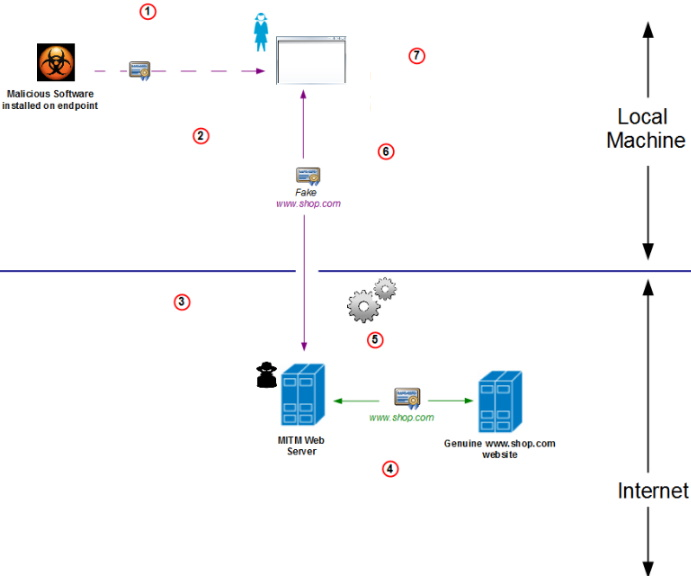
\includegraphics [width=15cm]{mitm_no_CISE.jpg}
	\caption[Man in the middle - Angriff auf SSL verschlüsselte Verbindungen]{MITM - Angriff auf SSL verschlüsselte Verbindungen}
	\label{fig:mitm_no_cise}
\end{figure}

\begin{enumerate} 
\item Im ersten Schritt muss der Angreifer ein eigenes Fake-Zertifikat (im folgenden \ac{mitm}-Zertifikat genannt) im Zertifikatsspeicher des Nutzers installieren. Dies kann eine Malware oder sonstige Fremdsoftware machen. Hat man als Angreifer phsysischen Zugriff zum Rechner, kann man dies innerhalb von wenigen Sekunden selbst machen, ohne dass der Nutzer davon etwas mitbekommt. Der \ac{mitm} - Angriff basiert auf diesem \ac{mitm}-Zertifikat, das von einem potenziellen Angreifer im Namen einer Webseite fälschlicherweise ausgestellt wurde. Ohne diesen Schritt funktioniert der Angriff nicht.
\item Der User möchte eine Verbindung zum Webshop (im Schaubild www.shop.com) aufbauen. Hierzu ruft er die Seite mit dem Präfix https:// auf im Glauben, eine sichere Verbindung aufbauen zu können, die von keinem Dritten mitgelesen werden kann. Der \ac{mitm} fängt die Anfrage ab und leitet ihn zu seinem eigenen Webserver weiter.
\newpage
\item Der Webserver erkennt einen \ac{https} - Request und entschlüsselt mit dem eigenen privaten Schlüssel. Dies kann er durch die Installation der Fake-Root-CA in Schritt 1. Dort wurde die Nachricht mit dem öffentlichen Schlüssel des Angreifers verschlüsselt und abgesendet.
\item Simultan baut der MITM-Webserver eine Verbindung zum echten Webshop auf und leitet die Daten des Nutzers jeweils in beide Richtungen weiter. Dabei simuliert er eine gewöhnliche Nutzeranfrage, die der Webshop nicht als fälschlich erkennen kann. Der User hingegen merkt nichts von dem Angreifer, da er die gewohnte (dies ist Standard) Webseite angezeigt bekommt und keine Annomalien erkennt.
\item Der gesamte Traffic, der eigentlich verschlüsselt sein sollte, kann vom \ac{mitm} mitgelesen, weitergeleitet oder manipuliert werden. Die Verbindung zwischen User und dem Webshop ist nicht sicher trotz \ac{https} Anzeige im Browser.
\item Die Response vom Webshop wird mit dem erstellten MITM-Zertifikat für www.shop.com verschlüsselt und an den User übertragen.
\item Der Browser markiert die Verbindung als sicher und unbedenklich.
\end{enumerate}

Der Nachteil für den Angreifer in diesem Szenario ist die zeitlich limitierte Möglichkeit eines Angriffs. Es muss also auf den initialen Request des Users gewartet werden, um dessen Daten abzufangen und den Prozess des Angriffs in Gang zu setzen. Wiederholungsangriffe (auch: Replay-Attacks) werden in diesem Szenario nicht verhindert. Der Angreifer muss womöglich demnach nicht einmal das Passwort im Klartext besitzen. Es genügt, den Hash und den Benutzernamen im Request abzufangen um diese dann in einem seperaten Aufruf vom eigenen Rechner an die selbe \ac{url} zu senden. Es handelt sich bei dieser Art des Angriffs um das Imitieren von Benutzereingaben durch einen Angreifer, bei der der Angreifer das Geheimnis nicht im Klartext kennt.

Durch den Zugang zum Dienst ist es dem Angreifer somit (je nach Implementierung) möglich, sensible Daten des Nutzers einzusehen, die nicht für ihn bestimmt sind. Die Frage nach der 'Relevanz' von sensiblen Daten sollte obsolet werden, wenn man an die Möglichkeiten denkt, die der Angreifer mit ihnen nun in der Hand hällt. Mit diesen könnte er den Nutzer zum Beispiel erpressen um an noch mehr Daten oder Geld des Nutzers zu kommen.

\subsection{Alternative Methoden}
Neben den bereits etablierten Methoden beschäftigt sich die Forschung mit alternativen Authentifizierungsverfahren wie der 'negative authentication' und der 'adaptive mult-factor authentication'. Was diese Verfahren für die Forschung bedeuten und inwiefern sie einen Vorteil bieten wird im Folgenden erläutert.

\textbf{Negative Authentication (NA)}

Bei der \ac{nas} wird die Useranfrage auf Invalidität statt auf Validität geprüft. Die Idee dahinter basiert auf dem 'Negative Selection Algorithm', welcher das menschliche Immunsystem als Insipriator verwendet. T - Helferzellen dienen hierbei der Unterscheidung von Entitäten im Körper nach 'körpereigen' (self) und 'körperfremd' (non-self). \cite{A11} \\

\begin{figure}[ht]
	\centering
	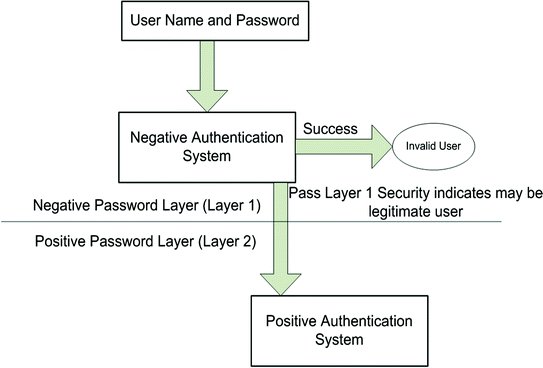
\includegraphics [width=15cm]{negative_password_architecture.png}
	\caption[Architektur zur Authentifizierung mit einem 'Negative Authentication System']{Architektur zur Authentifizierung mit einem 'Negative Authentication System'}
	\label{fig:negative_password_architecture}
\end{figure}

In der self-region sind die Passwortdaten beherrbergt. Diese Daten werden von der weitaus größeren non-self-region 'umschlossen', in der sich die Anti-Passwort-Detectoren befinden.
Während man \ac{nas} verwendet, ist es angebracht die Passwort-Profile und die Anti-Passwort-Profile auf zwei voneinander getrennten Servern zu bewahren. Dabei finden wie auf der Abbildung 2.2 zu sehen zwei Authentifizierungen statt. Bei der Ersten wird der Request mit der Datenmenge der Anti-Passwörter verglichen. Gibt es ein Match, ist der eingeggangene Request invalide. Auf diesem liegen die Detektoren für die Anti-Passwörter, die bei der Authentifizierung die Gülltigkeit der Anfrage erkennen, ähnlich wie die T-Helferzellen die Gülltigkeit von anderen Zellen im menschlichen Körper erkennen.

Dieser ''getrennte Server Ansatz`` für die Negativauthentikation besitzt gewisse Vorteile zu der Posoitivauthentifikation. Zunächst ein Mal ist es in der Lage bereits vor der eigentlichen Prüfung nach der Korrektheit des Passwortes invalide Requests abzufangen, die den zweiten Layer nie erreichen. Dies hat sich bereits als zielbringend erwiesen \cite{A14}. Außerdem sind die Daten des Nutzers hinter einem von außen nicht zu erreichenden Server versteckt, der nur mit dem ersten Layer kommuniziert. 'Guessing attacks' also Angriffe, die auf der Erratung von Passwörtern basieren, werden damit zu hoher Wahrscheinlichkeit verhindert \cite{A11}.

\textbf{Adaptive multi-factor-authentication (A-MFA)}

Da Nutzer durch mobile Technologien immer mehr Zugriff auf Online Services erhielten, entwickelte sich der Stand der Forschung immer mehr in Richtung verschiedener Authentifizierungsverfahren, unter denen der User eine Auswahl für sich treffen muss um seine Identität zu bestätigen \cite{A11}. Die Auswahl an Authentifizierungsfaktoren die dem Nutzer von Anwendungen präsentiert werden, entscheidet letzlich über die Performance von MFA's \cite{A11}. Daraus resultiert, dass die zufällige (oder Selbe) Auswahl von Verfahren für die MFA die Vertrauenswürdigkeit beeinträchtigen, da die Auswahl erratbar wird und bei entsprechenden Exploits auch unsicher. 

Die Auswahl der Verfahren findet zunächst aufgrund der Möglichkeiten eines Nutzers statt, demnach wird ermittelt welche Umgebung (welches Betriebssystem, welches Kommunikationsmedium und historische Daten) der Nutzer verwendet \cite{A15}. Um eine sichere Lösung für eine adaptive MFA zu entwickeln, muss die Erratbarkeit von dem Set an Authentifikationsmöglichkeiten verhindert werden. Dies bedeutet, dass es nicht möglich sein darf vordefinierte Muster für einen speziellen Nutzer mit einer speziellen Umgebung vorrauszusagen \cite{11}.

\section{Zielsetzung}
Passwörter können der allumfassenden sicheren Authentifikation nicht mehr gerecht werden. Es braucht weitere oder gänzlich andere Methoden, um die Identität eines Nutzers zu schützen. Die Menschheit benötigt einfache und unkomplizierte Methoden, die ihnen nicht das Gefühl geben allumfängliches technisches Know-How besitzen zu müssen, um die eigenen Daten im Internet zu schützen. Es sollte zum konsens werden, dass es bequeme Mechanismen für jeden Nutzer gibt. Je nach Gewichtung der Relevanz der Daten in den Kriterien Sicherheit, Bequemlichkeit und Datenschutz gibt es Möglichkeiten dies zu bewerkstelligen. Dies muss sowohl den Dienstbetreibern als auch dem Endnutzer bewusst werden. Nur die Erkenntnis über ein vorhandenes Problem kann zur Besserung führen und ist der erste Schritt. Nur so kann das Passwortproblem ein für alle Mal gelöst werden.

Ziel dieser Abschlussarbeit ist es eine Möglichkeit der Authentifikation zu spezifizieren, die im Jahre 2020 keine utopischen Szenarien beschreibt, die die Voraussetzungen für eine sichere, bequeme und datenarme Authentifikation erfüllt. Ziel ist es auch, den Leser in die Sicht des Angreifers auf Systeme einzuweisen, sodass im Idealfall automatische Schutzreaktionen wie das Wählen von sicheren Passwörtern hervorgerufen, wenn nicht sogar eine der beschriebenen FIDO2 Verfahren wie der erste oder sogar der zweite Faktor, verwendet werden. Der Prototyp soll die verschiedenen Authentifizierungsmöglichkeiten veranschaulischen und präsentieren, um dem Nutzer die Wahl auf eines der Verfahren zu erleichtern. Gleichzeitig ist eines der Hauptziele dieser Arbeit auch die Grenzen von 'modernen' Authentifizierungsverfahren aufzuzeigen und auf dessen Nachteile hinzuweisen. Inwiefern eine Kombination dieser vorhandenen Verfahren, Probleme löst und welche minderen Probleme dabei entstehen soll ausführlich erläutert werden. Jeder Nutzer besitzt persönliche Daten, an die kein Angreifer bzw. kein Dritter gelangen soll. Der Schutz dieser Daten sollte jedem Individuum selbst wichtig sein, um in den nächsten 5 bis 10 Jahren auf Besserung zu hoffen. Nicht nur technisch muss die Menscheit mit dem neuen digitalen Zeitalter umgehen und sich absichern können, sondern auch auf die menschliche Komponente muss von jedem selbst geachtet werden.

Dennoch sollte erwähnt sein, dass diese Arbeit nicht darauf abzielt jede mögliche vorhandene Authentifikationsstrategie zu durchleuchten. Erläutert werden die klassiche User-ID und Passwort Authentifikation und dem Gegenüber stehen die meistgenutzen Verfahren, die meist eher auf private Schlüssel, Besitz oder Biometrie setzen. Auch ist es ein Nicht-Ziel dieser Arbeit das Resultat auf eine einzige perfekte Lösung zu dezimieren und diese zum neuen Standard zu erklären. Viel mehr soll es dem Leser durch eine tabellarische Auflistung von Vor- und Nachteilen jeder Methodik selbst überlassen sein, welche Authentifikationsmethode ausgewählt wird.
